% Created by tikzDevice version 0.12.6 on 2024-08-01 12:50:17
% !TEX encoding = UTF-8 Unicode
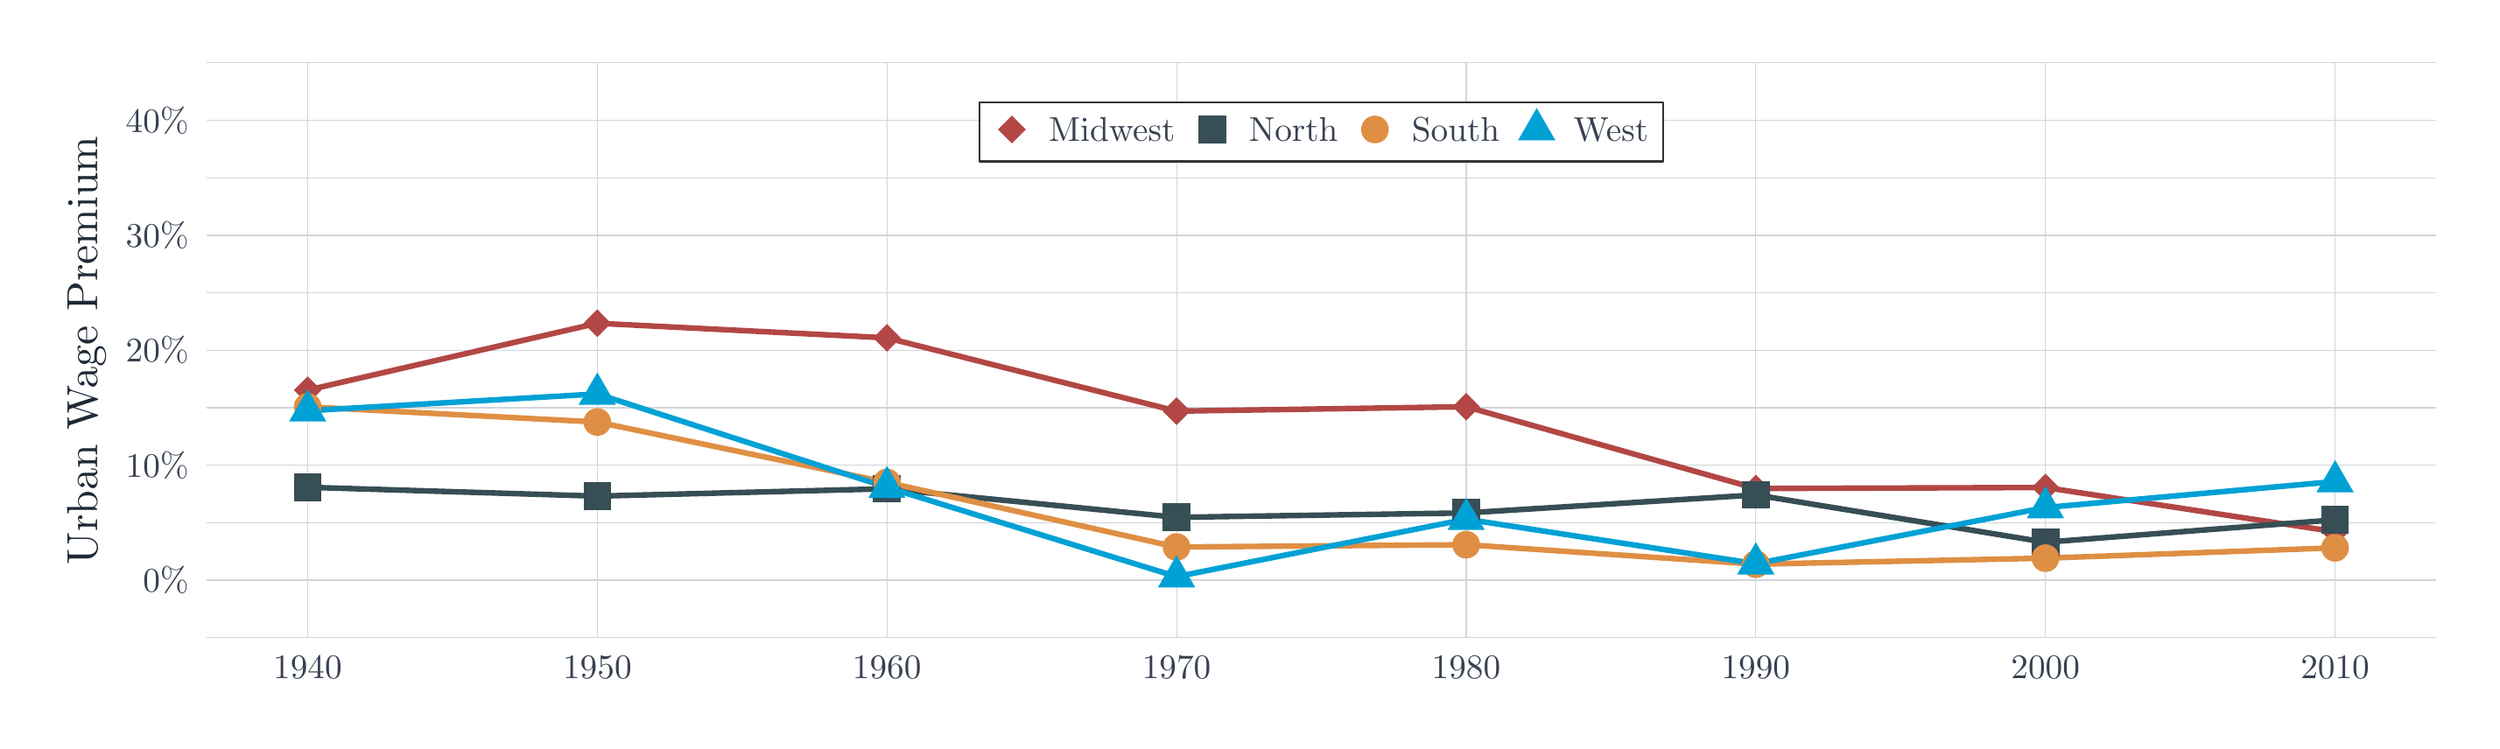
\begin{tikzpicture}[x=1pt,y=1pt]
\definecolor{fillColor}{RGB}{255,255,255}
\path[use as bounding box,fill=fillColor] (0,0) rectangle (1011.78,289.08);
\begin{scope}
\path[clip] (  0.00,  0.00) rectangle (1011.78,289.08);
\definecolor{drawColor}{RGB}{255,255,255}

\path[draw=drawColor,line width= 0.8pt,line join=round,line cap=round,fill=fillColor] (  0.00,  0.00) rectangle (1011.78,289.08);
\end{scope}
\begin{scope}
\path[clip] ( 75.16, 35.76) rectangle (995.78,273.08);
\definecolor{drawColor}{RGB}{255,255,255}
\definecolor{fillColor}{RGB}{255,255,255}

\path[draw=drawColor,line width= 0.8pt,line join=round,line cap=round,fill=fillColor] ( 75.16, 35.76) rectangle (995.78,273.08);
\definecolor{drawColor}{RGB}{209,213,219}

\path[draw=drawColor,line width= 0.4pt,line join=round] ( 75.16, 35.76) --
	(995.78, 35.76);

\path[draw=drawColor,line width= 0.4pt,line join=round] ( 75.16, 83.22) --
	(995.78, 83.22);

\path[draw=drawColor,line width= 0.4pt,line join=round] ( 75.16,130.69) --
	(995.78,130.69);

\path[draw=drawColor,line width= 0.4pt,line join=round] ( 75.16,178.15) --
	(995.78,178.15);

\path[draw=drawColor,line width= 0.4pt,line join=round] ( 75.16,225.62) --
	(995.78,225.62);

\path[draw=drawColor,line width= 0.4pt,line join=round] ( 75.16,273.08) --
	(995.78,273.08);

\path[draw=drawColor,line width= 0.4pt,line join=round] ( 75.16, 59.49) --
	(995.78, 59.49);

\path[draw=drawColor,line width= 0.4pt,line join=round] ( 75.16,106.95) --
	(995.78,106.95);

\path[draw=drawColor,line width= 0.4pt,line join=round] ( 75.16,154.42) --
	(995.78,154.42);

\path[draw=drawColor,line width= 0.4pt,line join=round] ( 75.16,201.88) --
	(995.78,201.88);

\path[draw=drawColor,line width= 0.4pt,line join=round] ( 75.16,249.35) --
	(995.78,249.35);

\path[draw=drawColor,line width= 0.4pt,line join=round] (117.01, 35.76) --
	(117.01,273.08);

\path[draw=drawColor,line width= 0.4pt,line join=round] (236.57, 35.76) --
	(236.57,273.08);

\path[draw=drawColor,line width= 0.4pt,line join=round] (356.13, 35.76) --
	(356.13,273.08);

\path[draw=drawColor,line width= 0.4pt,line join=round] (475.69, 35.76) --
	(475.69,273.08);

\path[draw=drawColor,line width= 0.4pt,line join=round] (595.25, 35.76) --
	(595.25,273.08);

\path[draw=drawColor,line width= 0.4pt,line join=round] (714.81, 35.76) --
	(714.81,273.08);

\path[draw=drawColor,line width= 0.4pt,line join=round] (834.37, 35.76) --
	(834.37,273.08);

\path[draw=drawColor,line width= 0.4pt,line join=round] (953.93, 35.76) --
	(953.93,273.08);
\definecolor{drawColor}{RGB}{178,71,69}

\path[draw=drawColor,line width= 2.3pt,line join=round] (117.01,137.98) --
	(236.57,165.58) --
	(356.13,159.55) --
	(475.69,129.29) --
	(595.25,131.11) --
	(714.81, 97.35) --
	(834.37, 97.75) --
	(953.93, 79.48);
\definecolor{drawColor}{RGB}{55,78,85}

\path[draw=drawColor,line width= 2.3pt,line join=round] (117.01, 97.85) --
	(236.57, 94.19) --
	(356.13, 97.23) --
	(475.69, 85.44) --
	(595.25, 87.25) --
	(714.81, 94.69) --
	(834.37, 75.15) --
	(953.93, 84.40);
\definecolor{drawColor}{RGB}{223,143,68}

\path[draw=drawColor,line width= 2.3pt,line join=round] (117.01,131.07) --
	(236.57,124.79) --
	(356.13, 99.85) --
	(475.69, 73.17) --
	(595.25, 74.13) --
	(714.81, 66.09) --
	(834.37, 68.57) --
	(953.93, 72.84);
\definecolor{drawColor}{RGB}{0,161,213}

\path[draw=drawColor,line width= 2.3pt,line join=round] (117.01,129.46) --
	(236.57,136.39) --
	(356.13, 97.84) --
	(475.69, 60.94) --
	(595.25, 84.67) --
	(714.81, 66.29) --
	(834.37, 89.48) --
	(953.93,100.21);
\definecolor{fillColor}{RGB}{178,71,69}

\path[fill=fillColor] (111.30,137.98) --
	(117.01,143.69) --
	(122.72,137.98) --
	(117.01,132.27) --
	cycle;
\definecolor{fillColor}{RGB}{55,78,85}

\path[fill=fillColor] (111.30, 92.13) --
	(122.72, 92.13) --
	(122.72,103.56) --
	(111.30,103.56) --
	cycle;
\definecolor{fillColor}{RGB}{223,143,68}

\path[fill=fillColor] (117.01,131.07) circle (  5.71);
\definecolor{fillColor}{RGB}{0,161,213}

\path[fill=fillColor] (117.01,138.34) --
	(124.70,125.02) --
	(109.32,125.02) --
	cycle;
\definecolor{fillColor}{RGB}{178,71,69}

\path[fill=fillColor] (230.86,165.58) --
	(236.57,171.30) --
	(242.28,165.58) --
	(236.57,159.87) --
	cycle;
\definecolor{fillColor}{RGB}{55,78,85}

\path[fill=fillColor] (230.86, 88.48) --
	(242.28, 88.48) --
	(242.28, 99.91) --
	(230.86, 99.91) --
	cycle;
\definecolor{fillColor}{RGB}{223,143,68}

\path[fill=fillColor] (236.57,124.79) circle (  5.71);
\definecolor{fillColor}{RGB}{0,161,213}

\path[fill=fillColor] (236.57,145.27) --
	(244.26,131.95) --
	(228.88,131.95) --
	cycle;
\definecolor{fillColor}{RGB}{178,71,69}

\path[fill=fillColor] (350.42,159.55) --
	(356.13,165.26) --
	(361.84,159.55) --
	(356.13,153.84) --
	cycle;
\definecolor{fillColor}{RGB}{55,78,85}

\path[fill=fillColor] (350.42, 91.52) --
	(361.84, 91.52) --
	(361.84,102.94) --
	(350.42,102.94) --
	cycle;
\definecolor{fillColor}{RGB}{223,143,68}

\path[fill=fillColor] (356.13, 99.85) circle (  5.71);
\definecolor{fillColor}{RGB}{0,161,213}

\path[fill=fillColor] (356.13,106.72) --
	(363.82, 93.40) --
	(348.44, 93.40) --
	cycle;
\definecolor{fillColor}{RGB}{178,71,69}

\path[fill=fillColor] (469.98,129.29) --
	(475.69,135.00) --
	(481.40,129.29) --
	(475.69,123.58) --
	cycle;
\definecolor{fillColor}{RGB}{55,78,85}

\path[fill=fillColor] (469.98, 79.73) --
	(481.40, 79.73) --
	(481.40, 91.15) --
	(469.98, 91.15) --
	cycle;
\definecolor{fillColor}{RGB}{223,143,68}

\path[fill=fillColor] (475.69, 73.17) circle (  5.71);
\definecolor{fillColor}{RGB}{0,161,213}

\path[fill=fillColor] (475.69, 69.82) --
	(483.38, 56.50) --
	(468.00, 56.50) --
	cycle;
\definecolor{fillColor}{RGB}{178,71,69}

\path[fill=fillColor] (589.54,131.11) --
	(595.25,136.82) --
	(600.96,131.11) --
	(595.25,125.40) --
	cycle;
\definecolor{fillColor}{RGB}{55,78,85}

\path[fill=fillColor] (589.54, 81.54) --
	(600.96, 81.54) --
	(600.96, 92.96) --
	(589.54, 92.96) --
	cycle;
\definecolor{fillColor}{RGB}{223,143,68}

\path[fill=fillColor] (595.25, 74.13) circle (  5.71);
\definecolor{fillColor}{RGB}{0,161,213}

\path[fill=fillColor] (595.25, 93.55) --
	(602.94, 80.23) --
	(587.56, 80.23) --
	cycle;
\definecolor{fillColor}{RGB}{178,71,69}

\path[fill=fillColor] (709.10, 97.35) --
	(714.81,103.06) --
	(720.52, 97.35) --
	(714.81, 91.64) --
	cycle;
\definecolor{fillColor}{RGB}{55,78,85}

\path[fill=fillColor] (709.10, 88.98) --
	(720.52, 88.98) --
	(720.52,100.40) --
	(709.10,100.40) --
	cycle;
\definecolor{fillColor}{RGB}{223,143,68}

\path[fill=fillColor] (714.81, 66.09) circle (  5.71);
\definecolor{fillColor}{RGB}{0,161,213}

\path[fill=fillColor] (714.81, 75.17) --
	(722.50, 61.85) --
	(707.12, 61.85) --
	cycle;
\definecolor{fillColor}{RGB}{178,71,69}

\path[fill=fillColor] (828.66, 97.75) --
	(834.37,103.46) --
	(840.08, 97.75) --
	(834.37, 92.04) --
	cycle;
\definecolor{fillColor}{RGB}{55,78,85}

\path[fill=fillColor] (828.66, 69.44) --
	(840.08, 69.44) --
	(840.08, 80.86) --
	(828.66, 80.86) --
	cycle;
\definecolor{fillColor}{RGB}{223,143,68}

\path[fill=fillColor] (834.37, 68.57) circle (  5.71);
\definecolor{fillColor}{RGB}{0,161,213}

\path[fill=fillColor] (834.37, 98.36) --
	(842.06, 85.04) --
	(826.68, 85.04) --
	cycle;
\definecolor{fillColor}{RGB}{178,71,69}

\path[fill=fillColor] (948.22, 79.48) --
	(953.93, 85.20) --
	(959.64, 79.48) --
	(953.93, 73.77) --
	cycle;
\definecolor{fillColor}{RGB}{55,78,85}

\path[fill=fillColor] (948.22, 78.69) --
	(959.64, 78.69) --
	(959.64, 90.11) --
	(948.22, 90.11) --
	cycle;
\definecolor{fillColor}{RGB}{223,143,68}

\path[fill=fillColor] (953.93, 72.84) circle (  5.71);
\definecolor{fillColor}{RGB}{0,161,213}

\path[fill=fillColor] (953.93,109.09) --
	(961.62, 95.77) --
	(946.24, 95.77) --
	cycle;
\end{scope}
\begin{scope}
\path[clip] (  0.00,  0.00) rectangle (1011.78,289.08);
\definecolor{drawColor}{RGB}{55,65,81}

\node[text=drawColor,anchor=base east,inner sep=0pt, outer sep=0pt, scale=  1.42] at ( 67.96, 54.59) {0\%};

\node[text=drawColor,anchor=base east,inner sep=0pt, outer sep=0pt, scale=  1.42] at ( 67.96,102.06) {10\%};

\node[text=drawColor,anchor=base east,inner sep=0pt, outer sep=0pt, scale=  1.42] at ( 67.96,149.52) {20\%};

\node[text=drawColor,anchor=base east,inner sep=0pt, outer sep=0pt, scale=  1.42] at ( 67.96,196.99) {30\%};

\node[text=drawColor,anchor=base east,inner sep=0pt, outer sep=0pt, scale=  1.42] at ( 67.96,244.45) {40\%};
\end{scope}
\begin{scope}
\path[clip] (  0.00,  0.00) rectangle (1011.78,289.08);
\definecolor{drawColor}{RGB}{55,65,81}

\node[text=drawColor,anchor=base,inner sep=0pt, outer sep=0pt, scale=  1.42] at (117.01, 18.76) {1940};

\node[text=drawColor,anchor=base,inner sep=0pt, outer sep=0pt, scale=  1.42] at (236.57, 18.76) {1950};

\node[text=drawColor,anchor=base,inner sep=0pt, outer sep=0pt, scale=  1.42] at (356.13, 18.76) {1960};

\node[text=drawColor,anchor=base,inner sep=0pt, outer sep=0pt, scale=  1.42] at (475.69, 18.76) {1970};

\node[text=drawColor,anchor=base,inner sep=0pt, outer sep=0pt, scale=  1.42] at (595.25, 18.76) {1980};

\node[text=drawColor,anchor=base,inner sep=0pt, outer sep=0pt, scale=  1.42] at (714.81, 18.76) {1990};

\node[text=drawColor,anchor=base,inner sep=0pt, outer sep=0pt, scale=  1.42] at (834.37, 18.76) {2000};

\node[text=drawColor,anchor=base,inner sep=0pt, outer sep=0pt, scale=  1.42] at (953.93, 18.76) {2010};
\end{scope}
\begin{scope}
\path[clip] (  0.00,  0.00) rectangle (1011.78,289.08);
\definecolor{drawColor}{RGB}{31,41,55}

\node[text=drawColor,rotate= 90.00,anchor=base,inner sep=0pt, outer sep=0pt, scale=  1.80] at ( 30.15,154.42) {Urban Wage Premium};
\end{scope}
\begin{scope}
\path[clip] (  0.00,  0.00) rectangle (1011.78,289.08);
\definecolor{drawColor}{gray}{0.20}
\definecolor{fillColor}{RGB}{255,255,255}

\path[draw=drawColor,line width= 0.8pt,line join=round,line cap=round,fill=fillColor] (394.47,232.37) rectangle (676.47,256.83);
\end{scope}
\begin{scope}
\path[clip] (  0.00,  0.00) rectangle (1011.78,289.08);
\definecolor{drawColor}{RGB}{255,255,255}
\definecolor{fillColor}{RGB}{255,255,255}

\path[draw=drawColor,line width= 0.8pt,line join=round,line cap=round,fill=fillColor] (400.47,238.37) rectangle (414.92,252.83);
\end{scope}
\begin{scope}
\path[clip] (  0.00,  0.00) rectangle (1011.78,289.08);
\definecolor{fillColor}{RGB}{178,71,69}

\path[fill=fillColor] (401.99,245.60) --
	(407.70,251.31) --
	(413.41,245.60) --
	(407.70,239.89) --
	cycle;
\end{scope}
\begin{scope}
\path[clip] (  0.00,  0.00) rectangle (1011.78,289.08);
\definecolor{drawColor}{RGB}{255,255,255}
\definecolor{fillColor}{RGB}{255,255,255}

\path[draw=drawColor,line width= 0.8pt,line join=round,line cap=round,fill=fillColor] (483.13,238.37) rectangle (497.58,252.83);
\end{scope}
\begin{scope}
\path[clip] (  0.00,  0.00) rectangle (1011.78,289.08);
\definecolor{fillColor}{RGB}{55,78,85}

\path[fill=fillColor] (484.65,239.89) --
	(496.07,239.89) --
	(496.07,251.31) --
	(484.65,251.31) --
	cycle;
\end{scope}
\begin{scope}
\path[clip] (  0.00,  0.00) rectangle (1011.78,289.08);
\definecolor{drawColor}{RGB}{255,255,255}
\definecolor{fillColor}{RGB}{255,255,255}

\path[draw=drawColor,line width= 0.8pt,line join=round,line cap=round,fill=fillColor] (550.35,238.37) rectangle (564.80,252.83);
\end{scope}
\begin{scope}
\path[clip] (  0.00,  0.00) rectangle (1011.78,289.08);
\definecolor{fillColor}{RGB}{223,143,68}

\path[fill=fillColor] (557.58,245.60) circle (  5.71);
\end{scope}
\begin{scope}
\path[clip] (  0.00,  0.00) rectangle (1011.78,289.08);
\definecolor{drawColor}{RGB}{255,255,255}
\definecolor{fillColor}{RGB}{255,255,255}

\path[draw=drawColor,line width= 0.8pt,line join=round,line cap=round,fill=fillColor] (617.13,238.37) rectangle (631.59,252.83);
\end{scope}
\begin{scope}
\path[clip] (  0.00,  0.00) rectangle (1011.78,289.08);
\definecolor{fillColor}{RGB}{0,161,213}

\path[fill=fillColor] (624.36,254.48) --
	(632.05,241.16) --
	(616.67,241.16) --
	cycle;
\end{scope}
\begin{scope}
\path[clip] (  0.00,  0.00) rectangle (1011.78,289.08);
\definecolor{drawColor}{RGB}{55,65,81}

\node[text=drawColor,anchor=base west,inner sep=0pt, outer sep=0pt, scale=  1.42] at (422.92,240.70) {Midwest};
\end{scope}
\begin{scope}
\path[clip] (  0.00,  0.00) rectangle (1011.78,289.08);
\definecolor{drawColor}{RGB}{55,65,81}

\node[text=drawColor,anchor=base west,inner sep=0pt, outer sep=0pt, scale=  1.42] at (505.58,240.70) {North};
\end{scope}
\begin{scope}
\path[clip] (  0.00,  0.00) rectangle (1011.78,289.08);
\definecolor{drawColor}{RGB}{55,65,81}

\node[text=drawColor,anchor=base west,inner sep=0pt, outer sep=0pt, scale=  1.42] at (572.80,240.70) {South};
\end{scope}
\begin{scope}
\path[clip] (  0.00,  0.00) rectangle (1011.78,289.08);
\definecolor{drawColor}{RGB}{55,65,81}

\node[text=drawColor,anchor=base west,inner sep=0pt, outer sep=0pt, scale=  1.42] at (639.59,240.70) {West};
\end{scope}
\end{tikzpicture}
